% Dit werk is gelicenseerd onder de licentie Creative Commons Naamsvermelding-GelijkDelen 4.0 Internationaal. Ga naar http://creativecommons.org/licenses/by-sa/4.0/ om een kopie van de licentie te kunnen lezen.
\chapter{Open-kanaalstroming}
\label{sec:Kanaalstroming}

%%%%%%%%%%%%%%%%%%%%%%%%%%%%%%%%%%%%%%%%%%%%%%%%%%%%%%%%%%%%%%%%%%%%%%%%%%%%%%%%%%%%%
	\section{Inleiding}
	\label{sec:Kanaalstroming Inleiding}
Veel van de stromingen die we in het dagelijks leven tegenkomen hebben een vrij oppervlak. Hiermee wordt bedoeld dat een deel van het vloeistof oppervlak grenst aan een ander fluïdum. Vaak is dit ander fluïdum de lucht in de atmosfeer. Er wordt gesproken over vrij oppervlak stroming (E: free surface flow) aangezien het oppervlak van de vloeistof vrij is om te vervormen.

Een interessante subsectie van de vrije oppervlakte stromingen is de kanaal stroming. Hier stroomt een vloeistof in een kanaal waarvan één dimensie veel groter is dan de andere 2 en waar een vrij oppervlak ontstaat. Denk maar aan de stroming van beken en rivieren, kanalen (vandaar de naam) of zelfs leidingen die niet volledig gevuld zijn (Figuur \ref{fig:Open_kanaal_doorsnedes}). 
\begin{figure}[htb]
	\centering
	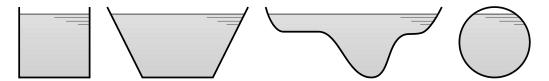
\includegraphics{fig/kanaalstroming/Open_kanaal_doorsnedes}
	\caption{Voorbeelden van doorsnedes van open kanalen}
	\label{fig:Open_kanaal_doorsnedes}
\end{figure}

De beweging van deze stromingen wordt voornamelijk veroorzaakt door de zwaartekracht. In de volgende secties zullen we enkele basisbegrippen noodzakelijk voor de analyse van de stroming in open kanalen afleiden of definiëren.

%%%%%%%%%%%%%%%%%%%%%%%%%%%%%%%%%%%%%%%%%%%%%%%%%%%%%%%%%%%%%%%%%%%%%%%%%%%%%%%%%%%%%
	\section{Oppervlaktegolven}
	\label{sec:Oppervlaktegolven}
	
Beschouw een kanaal met breedte $b$  waarin een een golf met een kleine uitwijking $\Delta y$ ten opzichte van de diepte van het kanaal $y$ zich voortplant. De golf beweegt met een nog onbekende snelheid $c$. Deze stroming kunnen we als stationair beschouwen indien we een controlevolume kiezen dat met de golf mee beweegt zoals in \ref{fig:Golfsnelheid}. We kiezen het controlevolume zo dat de ene zijde overeenkomt met de top van de golf en de andere zijde met de ongestoorde vloeistof.
\begin{figure}[htb]
	\centering
	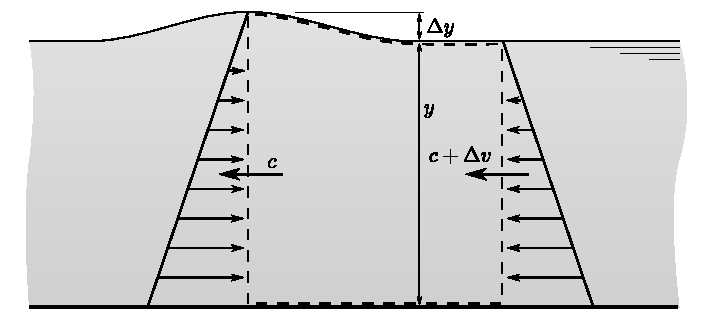
\includegraphics{fig/kanaalstroming/Golfsnelheid}
	\caption{Stationair controlevolume dat meebeweegt met een golf met een kleine uitwijking}
	\label{fig:Golfsnelheid}
\end{figure}
Door de beweging van het controlevolume is het alsof er aan de linkerzijde een gemiddelde stroomsnelheid, gelijk aan de golfsnelheid $c$ heerst. Aangezien aan de rechterzijde de hoogte lager is zal hier de gemiddelde snelheid groter zijn $c+\Delta v$. Schrijven we nu de vergelijking van behoud van massa uit:
\begin{equation}
	0 = (c+\Delta v) b y - c b (y+\Delta y)
\end{equation}
Hieruit kunnen we de golfsnelheid bepalen als:
\begin{equation}
	c = y \frac{\Delta v}{\Delta y}
	\label{eqn:golfsnelheid behoud van massa}
\end{equation}

We kunnen ook behoud van impuls uitschrijven in de voortplantingsrichting van de golf. De enige krachten die op het controlevolume inwerken zijn de drukkrachten aan de linker en rechterzijde:
\begin{equation}
	\frac{1}{2}\rho g (y+\Delta y)^2 b - \frac{1}{2}\rho g y^2 b = \rho b (y+\Delta y) c (c+\Delta v-c)
\end{equation}
Na uitwerking en deling door $\rho b \Delta y^2$ en herschikking wordt dit:
\begin{equation}
	 g \left(\frac{y}{\Delta y} + \frac{1}{2}\right)  = c \left(\frac{y}{\Delta y} + 1\right)\frac{\Delta v}{\Delta y}
\end{equation}
Hieruit kunnen we de verhouding van snelheidsverandering ten opzichte van de hoogteverandering bepalen:
\begin{equation}
	\frac{\Delta v}{\Delta y} = \frac{g}{c} \frac{\frac{y}{\Delta y} + \frac{1}{2}}{\frac{y}{\Delta y} + 1}
\end{equation}
Als nu $\Delta y$ veel kleiner is dan $y$ dan is de verhouding $\frac{\frac{y}{\Delta y} + \frac{1}{2}}{\frac{y}{\Delta y} + 1}$ ongeveer gelijk aan 1. Dus:
\begin{equation}
	\frac{\Delta v}{\Delta y} = \frac{g}{c}
\end{equation}
Indien we deze uitdrukking invullen in (\ref{eqn:golfsnelheid behoud van massa}) krijgen we:
\begin{equation}
	c = \sqrt{g y}
	\label{eqn:golfsnelheid ondiep}
\end{equation}

De golfsnelheid van een kleine golf is dus enkel afhankelijk van de diepte van het kanaal en de valversnelling en niet van de dichtheid van het fluïdum.

De uitwerking hierboven is enkel geldig voor een alleenstaande golf met een zeer kleine uitwijking. Wanneer verschillende golven met een bijvoorbeeld een sinusoïdaal profiel na elkaar beschouwd worden wordt de uitwerking veel complexer. De golfsnelheid wordt dan niet alleen afhankelijk van de diepte maar ook van de golflengte $\lambda$ (de afstand tussen 2 golf toppen) \cite{Henderson1966}. Hieruit volgt dat bovenstaande uitdrukking (\ref{eqn:golfsnelheid ondiep}) voor de golfsnelheid enkel geldig is wanneer de golflengte veel groter is dan de diepte ($\frac{\lambda}{y} > 20$, dus een enkele golf). Wanneer de golflengte in dezelfde grootteorde of kleiner is dan de diepte $\frac{\lambda}{y} < 3$ wordt de golfsnelheid benaderd door:
\begin{equation}
	c = \sqrt{\frac{g \lambda}{2\pi}}
	\label{eqn:golfsnelheid diep}
\end{equation}

Met geavanceerde uitdrukkingen van de golfsnelheid in functie van de diepte en golflengte is het mogelijk met behulp van Fourierreeksen zeer ingewikkelde golfprofielen te beschrijven.

%%%%%%%%%%%%%%%%%%%%%%%%%%%%%%%%%%%%%%%%%%%%%%%%%%%%%%%%%%%%%%%%%%%%%%%%%%%%%%%%%%%%
	\section{Energetische beschouwingen bij open kanaal stroming}
	\label{sec:Energetische beschouwingen bij open kanaal stroming}
Beschouw een stationaire uniforme stroming in een eenvoudig rechthoekig kanaal met een bepaalde helling (Figuur \ref{fig:Open_kanaal_bernoulli}). Noem $z$ de hoogte tot de bodem van het kanaal ten opzichte van een bepaalde referentie en $y$ de verticale afstand van het vloeistof oppervlak tot de bodem.
\begin{figure}[htb]
	\centering
	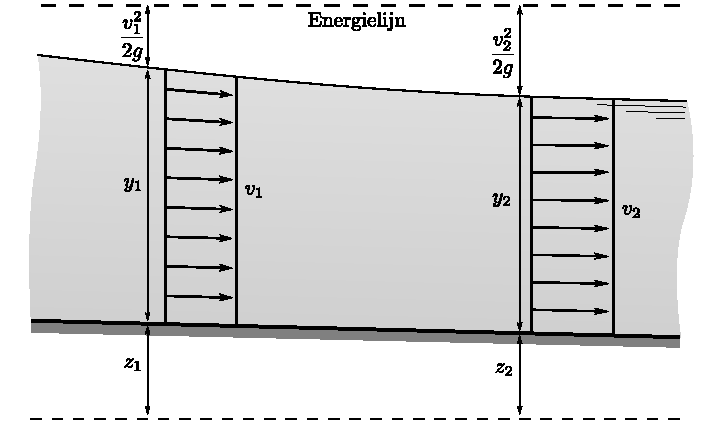
\includegraphics{fig/kanaalstroming/Open_kanaal_bernoulli}
	\caption{Stationaire uniforme stroming in een open kanaal met energielijnen}
	\label{fig:Open_kanaal_bernoulli}
\end{figure}
Indien de stroming niet-viskeus en niet-samendrukbaar is, kunnen we tussen 2 punten op de bodem van het kanaal de vergelijking van Bernoulli uitschrijven:
\begin{equation}
	\frac{p_1}{\rho g} + \frac{v_1^2}{2 g} + z_1 = \frac{p_2}{\rho g} + \frac{v_2^2}{2 g} + z_2
\end{equation}
De druk in het kanaal zal voornamelijk veroorzaakt worden door hydrostatische druk. De druk onderaan het kanaal kunnen we dus schrijven als $p = \rho g y$. Dus:
\begin{equation}
	y_1 + \frac{v_1^2}{2 g} + z_1 = y_2 + \frac{v_2^2}{2 g} + z_2
\end{equation}
In de bovenstaande vergelijking kunnen de eerste twee termen in het linker en rechter lid op een gegeven positie in het kanaal veranderen. De hoogte van het kanaal kan dit uiteraard niet. Het is nu interessant om de eerste twee termen te bundelen. Deze term wordt de \emph{specifieke energie} genoemd. De vergelijking van Bernoulli voor een open kanaal wordt dan:
\begin{equation}
	E_1 + z_1 = E_2 + z_2
\end{equation}
Met de specifieke energie $E$ gedefinieerd als:
\begin{equation}
	E = y + \frac{v^2}{2 g}
\end{equation}
Wanneer er geen viskeuze verliezen zijn zal dus de som van de specifieke energie en de hoogte van de bodem van het kanaal constant blijven.

De specifieke energie is enkel afhankelijk van de diepte van de stroming en de stroomsnelheid. Voor een kanaal met gegeven afmetingen zijn deze echter niet onafhankelijk. Aangezien het debiet constant is in het kanaal zal indien de snelheid stijgt, de hoogte dalen. De breedte van het kanaal $b$ speelt hier echter ook een rol. We kunnen dus de specifieke energie herschrijven in functie van het debiet per eenheid van breedte van het kanaal $q = \dot{V}/b$:
\begin{equation}
	E = y + \frac{q^2}{2 g y^2}
\end{equation}
Voor een kanaal met constante breedte zal $q$ constant blijven. We kunnen dus een diagram maken van de diepte in functie van de specifieke energie, het specifieke energie diagram (Figuur \ref{fig:Specifieke_energie_diagram}).
\begin{figure}[htb]
	\centering
	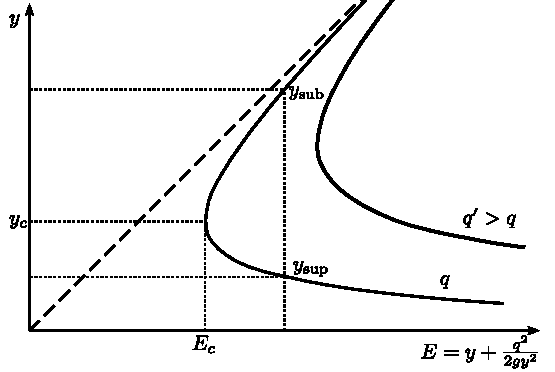
\includegraphics{fig/kanaalstroming/Specifieke_energie_diagram}
	\caption{Het specifieke energie diagram voor 2 verschillende debieten}
	\label{fig:Specifieke_energie_diagram}
\end{figure}
Op dit diagram zijn een aantal interessante punten aan te duiden. Vooreerst zien we dat bij een bepaald debiet niet alle waarden van specifieke energie mogelijk zijn. De specifieke energie heeft bij een bepaalde vloeistof hoogte een minimum. Deze diepte noemen we de kritische diepte $y_c$, de stroming bij de \emph{kritische diepte} noemen we \emph{kritische stroming}. We zien ook dat het diagram 2 asymptoten heeft. Voor grote dieptes wordt de specifieke energie gelijk aan de diepte, de snelheid streeft dus naar 0. Voor kleine dieptes evolueert de specifieke energie zelf naar 0. Voor waarden hoger dan de minimale specifieke energie zien we ook dat er telkens 2 mogelijke vloeistof hoogtes zijn (als je de vergelijking bekijkt zijn het er 3 maar één hiervan is steeds negatief en dus niet fysisch).

		\subsection{Kritische stroming}
Laten we nu de kritische diepte zoeken. Het minimum van de specifieke energie kunnen we vinden door zijn afgeleide naar de diepte gelijk aan 0 te stellen en dit op te lossen naar de diepte $y$.
\begin{equation}
	\frac{\diff E}{\diff y} = 1 - \frac{q^2}{g y^3} = 0
\end{equation}
Deze vergelijking is eenvoudig op te lossen naar $y$:
\begin{equation}
	y_c = \left( \frac{q^2}{g} \right)^{1/3}
\end{equation}
De snelheid bij kritische stroming $v_c$ kunnen we nu bepalen uit de uitdrukking voor het debiet $q = v_c y_c$. 
\begin{equation}
	y_c^3 = \frac{v_c^2 y_c^2}{g}
\end{equation}
Dus wordt de kritische snelheid:
\begin{equation}
	v_c = \sqrt{g y_c}
\end{equation}
Deze uitdrukking zijn we al eens tegengekomen, het is namelijk de voortplantingssnelheid van een oppervlakte golf met een grote golflengte (\ref{eqn:golfsnelheid ondiep}). We kunnen dus zeggen dat wanneer de stroomsnelheid  $v$ gelijk is aan de golfsnelheid $c$ we spreken over kritische stroming. Wanneer de stroomsnelheid lager is dan de golfsnelheid spreken we over \emph{sub-kritische stroming}. De diepte is dan groter dan de kritische diepte.  Wanneer de stroomsnelheid hoger is dan de golfsnelheid spreken we over \emph{super-kritische stroming}.  De diepte is dan kleiner dan de kritische diepte.

We kunnen nu ook een dimensieloos getal vormen door de de snelheid te delen door de kritische snelheid $\frac{v}{v_c}$. Ook deze uitdrukking zijn we reeds eerder tegengekomen, het is namelijk het Froude getal (\ref{eqn:Dimensieloze getallen}):
\begin{equation}
	\text{Fr} = \dfrac{v}{\sqrt{g y}}
\end{equation}
De betekenis ervan wordt nu ook duidelijker. Het Froude getal is de verhouding van de traagheidskrachten ten opzichte van de zwaartekracht, of de snelheid, die gerelateerd kan worden aan de traagheidskracht, ten opzichte van de golfsnelheid, die gerelateerd kan worden aan de zwaartekracht. Bij een Froude getal van 1 hebben we kritische stroming en zullen de traagheidskrachten en zwaartekracht elkaar in evenwicht houden. Bij een Froude getal groter dan 1 spreken we over super-kritische stroming en overheersen de traagheidskrachten. Bij een Froude getal kleiner dan 1 spreken we over sub-kritische stroming en overheerst de zwaartekracht.

	\section{Veranderingen in diepte bij verschillende stromingstypes}
Een interessante vraag is hoe de hoogte van het vloeistofoppervlak in een kanaal zal reageren op een verandering van hoogte is het kanaal. Beschouw hiervoor een eenvoudig kanaal met stationaire stroming waarvan de bodem een plotse stijging ondervindt (Figuur \ref{fig:Open_kanaal_bodemstijging_subkritisch}). 
\begin{figure}[htb]
	\centering
	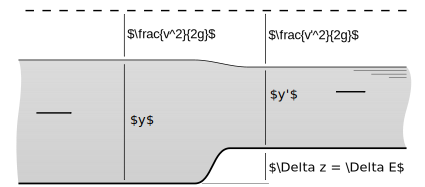
\includegraphics{fig/kanaalstroming/Open_kanaal_bodemstijging_subkritisch}
	\caption{Een plotse stijging van de bodem in een subkritische stroming veroorzaakt een daling van de diepte.}
	\label{fig:Open_kanaal_bodemstijging_subkritisch}
\end{figure}
We kunnen deze situatie analyseren met behulp van het specifieke energie diagram (Figuur \ref{fig:Specifieke_energie_diagram_bodemstijging}).

\begin{figure}[htb]
	\centering
	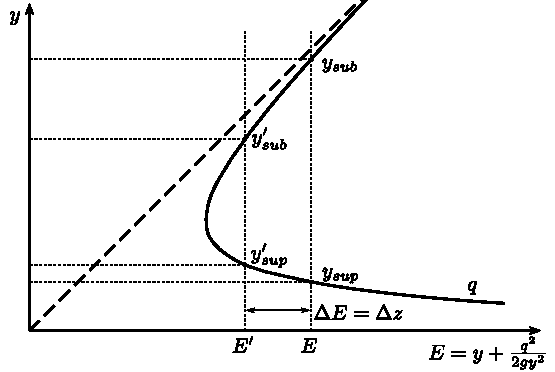
\includegraphics{fig/kanaalstroming/Specifieke_energie_diagram_bodemstijging}
	\caption{Specifieke energie diagram voor een plotse stijging van de hoogte van de bodem van een kanaal.}
	\label{fig:Specifieke_energie_diagram_bodemstijging}
\end{figure}

Het debiet door het kanaal voor en na de verhoging zal niet veranderen, $q$ is dus constant en we kunnen dus enkel op één curve bewegen. We kunnen veronderstellen dat de hoogte verandering bijna geen energieverliezen met zich meebrengt, de totale energie zal dus constant blijven, aangezien de hoogte $z$ stijgt moet dan de specifieke energie $E$ dalen. We bewegen ons dus naar links in het specifieke energie diagram van $E$ naar $E'$

Indien de stroming sub-kritisch is, bevinden we ons in het bovenste been van het specifieke energie diagram. Een stijging van de bodem zal dus leiden tot een daling van de vloeistof hoogte. Dit gaat steeds gepaard met een stijging van de snelheid.

Indien de stroming superkritisch is, bevinden we ons in het onderste been van het specifieke energie diagram. Een stijging van de bodem zal nu een stijging van de diepte en een daling van de snelheid veroorzaken (Figuur \ref{fig:Open_kanaal_bodemstijging_superkritisch}). 
\begin{figure}[htb]
	\centering
	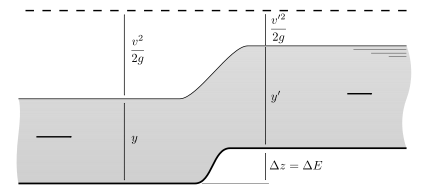
\includegraphics{fig/kanaalstroming/Open_kanaal_bodemstijging_superkritisch}
	\caption{Een plotse stijging van de bodem in een superkritische stroming veroorzaakt een stijging van de diepte.}
	\label{fig:Open_kanaal_bodemstijging_superkritisch}
\end{figure}

	\subsection{Verandering van stromingstype}
Uit de voorgaande beschouwingen kunnen we afleiden dat voor een subkritische stroming een verhoging van de bodem tot een bepaalde hoogte ervoor zal zorgen dat de de stroming kritisch wordt. Indien na de verhoging de bodem terug zal dalen ontstaat er een superkritische stroming (Figuur \ref{fig:Open_kanaal_subkritisch_naar_superkritisch}). De overgang van subkritische naar superkritische stroming gebeurt vrijwel zonder verliezen.

De overgang van superkritische stroming naar subkritische stroming verloopt echter anders. Wanneer door bijvoorbeeld een obstructie stroomafwaarts van een superkritische stroming de stroming terug subkritisch wordt ontstaat er \emph{hydraulische sprong} (E: Hydraulic jump). De diepte van de stroming zal hier plots stijgen en golven en wervelingen zullen terugklappen op de aankomende stroming (Figuur \ref{fig:Open_kanaal_subkritisch_naar_superkritisch}). 
\begin{figure}[htb]
	\centering
	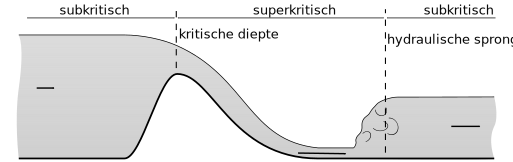
\includegraphics{fig/kanaalstroming/Open_kanaal_subkritisch_naar_superkritisch}
	\caption{De overgang van subkritische naar superkritische stroming gebeurt zonder veel energieverliezen terwijl de overgang van superkritische naar subkritische stroming gepaard gaat met een hydraulische sprong met grote energieverliezen.}
	\label{fig:Open_kanaal_subkritisch_naar_superkritisch}
\end{figure}

In een hydraulische sprong zal door de sterke werveling veel energie gedissipeerd worden. Dit kan nuttig zijn wanneer bijvoorbeeld een stroming te veel energie bevat. Zou men een superkritische stroming over een zacht materiaal laten stromen dan zal door de hoge snelheid dit materiaal snel weg eroderen. Indien men ervoor kan zorgen dat er een hydraulische sprong optreed voor het zachte materiaal zal een groot deel van de energie door viskeuze krachten gedissipeerd worden terwijl de snelheid van de stroming zal dalen en het gevaar voor erosie afneemt.
	
In \cite{Chaudhry2007} worden bovenstaande concepten evenals meer geavanceerde onderwerpen zeer duidelijk beschreven. Geïnteresseerde lezers worden dan ook hier naar verwezen.